\newpage
\section{Αρχιτεκτονική σχεδίαση} \label{section:3-7-architecture-design}

Σε αυτήν την ενότητα περιγράφεται η αρχιτεκτονική του συστήματος, όπως προέκυψε από την επιλεγμένη τεχνολογική στοίβα και τις προαναφερθείσες απαιτήσεις του. Θα πρέπει να σημειωθεί ότι η παρουσιαζόμενη αρχιτεκτονική είναι πρώιμη και δεν αποτελεί την τελική υλοποίηση της πλατφόρμας, η οποία περιγράφεται στο κεφάλαιο \ref{chapter:4-application-implementation}. 

Συνοπτικά, η αρχιτεκτονική του συστήματος αποτυπώνεται στο παρακάτω διάγραμμα:

\begin{figure}[H]
    \centering
    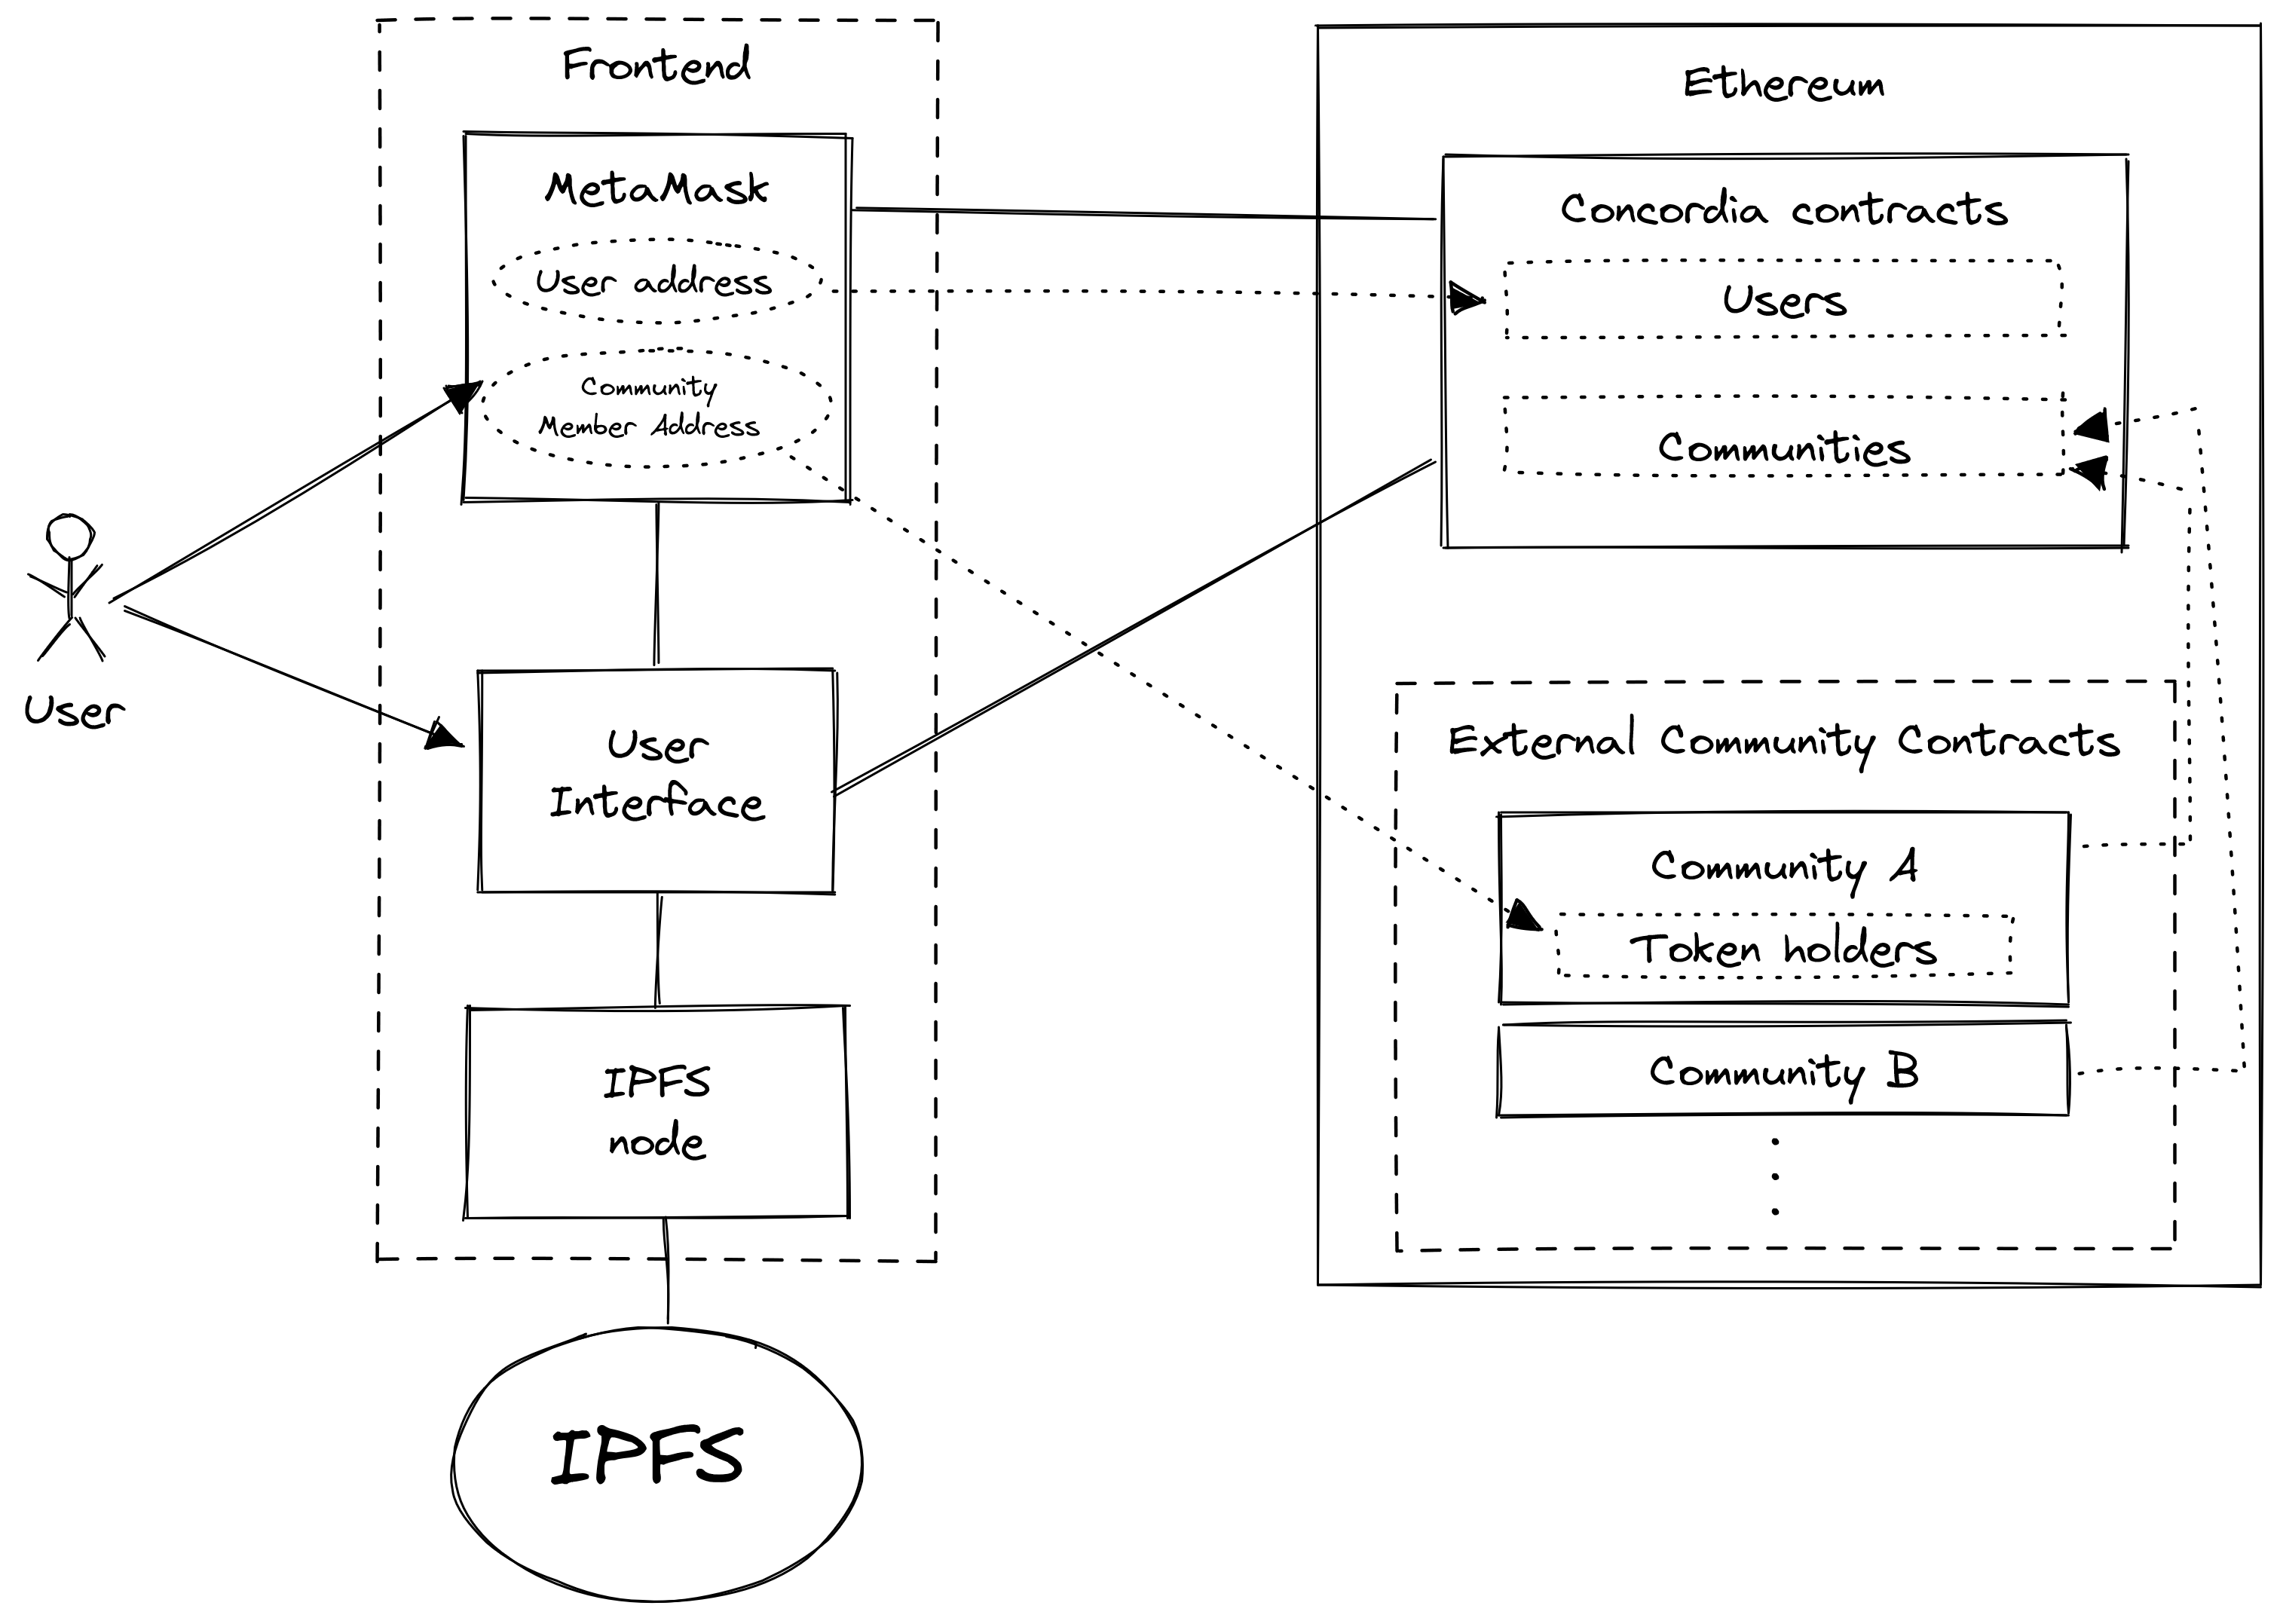
\includegraphics[width=\textwidth]{assets/figures/chapter-3/3.7.architecture-design}
    \caption{Αρχιτεκτονική του συστήματος (στάδιο σχεδίασης)}
\end{figure}

\vspace{\baselineskip}

Αξίζει να σημειωθούν τα εξής:

\begin{itemize}
    \item Ο κώδικας του frontend εκτελείται αποκλειστικά στο σύστημα του χρήστη, χωρίς να απαιτείται κάποιος εξυπηρετητής. Δηλαδή, ο χρήστης αρκεί απλά να έχει τον κώδικα αποθηκευμένο στον υπολογιστή του.
    \item Ο χρήστης αλληλεπιδρά άμεσα με το UI και το MetaMask. Το MetaMask αποτελεί browser add-on, το οποίο διαχειρίζεται τα ιδιωτικά κλειδιά Ethereum του χρήστη και πραγματοποιεί τις συναλλαγές του τελευταίου με τα smart contract. Στην προκειμένη περίπτωση, περιέχει τα κλειδιά που σχετίζονται αφενός με τη διεύθυνση με την οποία ο χρήστης εγγράφεται στην πλατφόρμα, αφετέρου με τις διευθύνσεις που περιέχουν τα token των κοινοτήτων στις οποίες ανήκει και έχει δικαιώματα ψήφου.
    \item Στο frontend εκτελείται στο παρασκήνιο ένας κόμβος για το IPFS. Αυτός συνδέεται με άλλους κατάλληλους κόμβους, διαμοιράζοντας τον κύριο όγκο των δεδομένων της εφαρμογής (π.χ. του περιεχομένου των μηνυμάτων).
    \item Τέλος, στο Ethereum blockchain υπάρχουν τόσο τα contract της εφαρμογής, όσο και τα εξωτερικά contract που παρέχουν τα token των κοινοτήτων. Τα μεν λειτουργούν ως το σημείο αναφοράς της εφαρμογής, επί του οποίου εκτελούνται οι ενέργειες και αποθηκεύονται οι μεταβλητές που είναι απολύτως απαραίτητες για τη λειτουργία της πλατφόρμας (π.χ. εγγεγραμμένοι χρήστες, δημιουργημένες κοινότητες). Τα δε δημιουργούνται από εξωτερικές οντότητες, οι οποίες ορίζουν κατά τη βούλησή τους τον ακριβή τρόπο δημιουργίας και διαμοιρασμού των token τους στους χρήστες.
\end{itemize}